\documentclass[simplex.tex]{subfiles}
% NO NEED TO INPUT PREAMBLES HERE
% packages are inherited; you can compile this on its own

\onlyinsubfile{
\title{NeuroData SIMPLEX Report: Subfile}
}

\begin{document}
\onlyinsubfile{
% \maketitle
\thispagestyle{empty}

% The following report documents the progress made by the labs of Randal~Burns and Joshua~T.~Vogelstein at Johns Hopkins University towards goals set by the DARPA SIMPLEX grant.

%%%% Table of Contents
% \tableofcontents

%%%% Publications
\bibliographystyle{IEEEtran}
\begin{spacing}{0.5}
% \section*{Publications, Presentations, and Talks}
%\vspace{-20pt}
\nocite{*}
{\footnotesize	\bibliography{simplex}}
\end{spacing}
%%%% End Publications
}

\subsection{LOL}

%We have proven the conditions under which LOL outperforms PCA.
%Specifically, PCA only outperforms LOL is we store enough eigenvectors
%such that the $d^\text{th}$ LOL outperforms PCA whenever the difference of the means
%and the first $d$ eigenvectors contain less information than the $(d + 1)^{\text{th}}$
%eigenvector.  The proof utilizes Chernoff divergences. More
%specifically, we can compute the Chernoff Information that one
%distribution has about another.  Thus, for a given low-dimensional
%projection, we can evaluate how far  $F_0$ and  $F_1$ are from one another, which
%determines the induced Bayes optimal error rate. The settings for which
%PCA outperforms LOL are quite pathological.


As you may recall from last month, we successfully proved that LOL outperforms PCA essentially always when performing a linear dimensionality reduction prior to classification.  This month we generate simulation results supporting those theoretical claims (see Figure \ref{fig:LOL})



\begin{figure}[h!]
\begin{cframed}
\centering
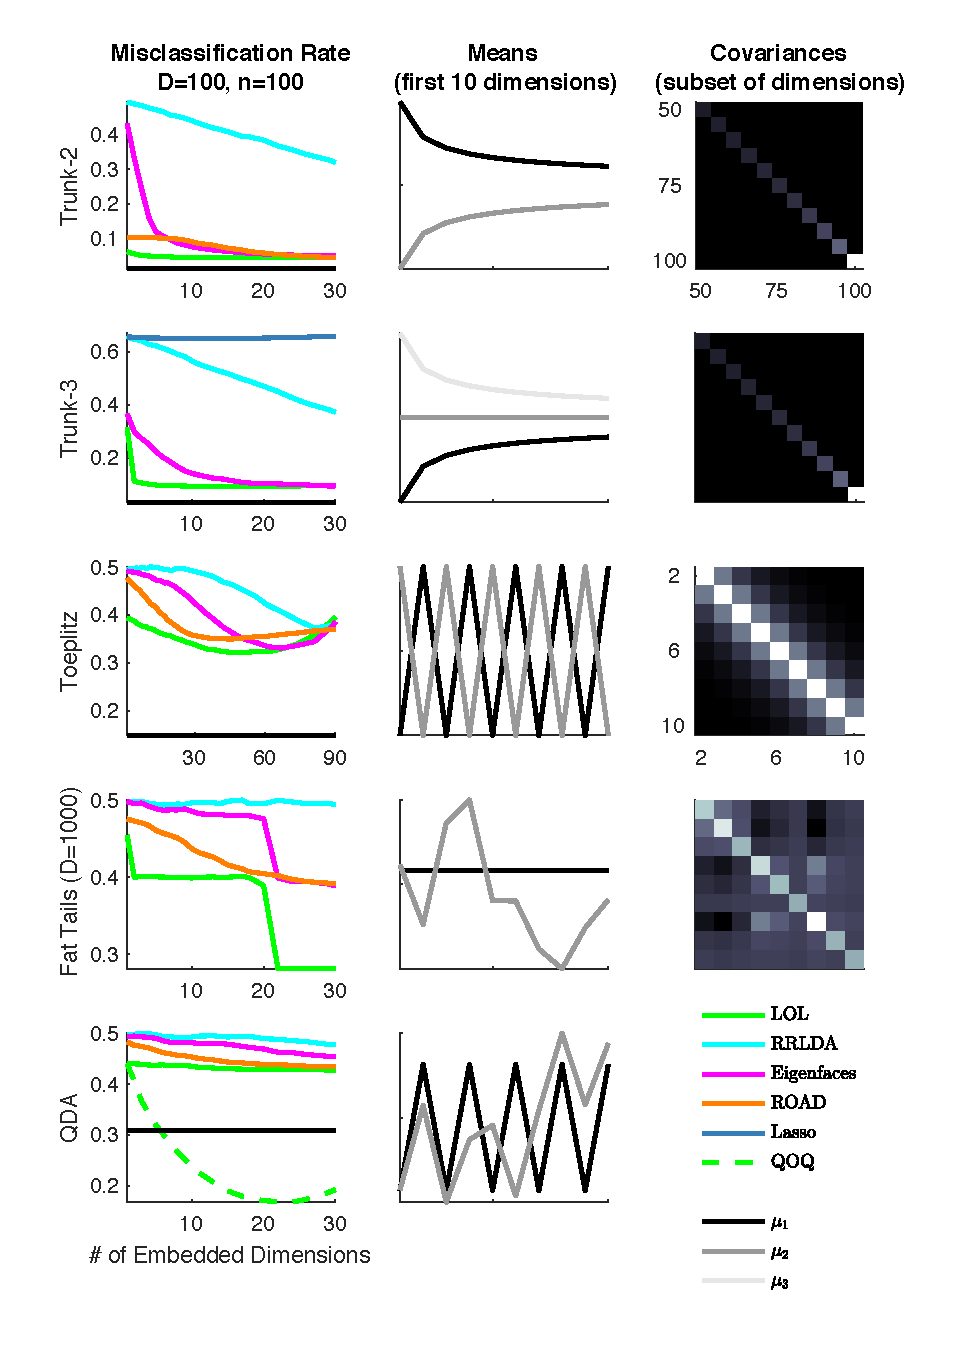
\includegraphics[width=0.7\textwidth]{../../figs/plot_all.pdf}
\caption{
LOL outperforms other linear classifiers in a wide variety of settings, including those for which we have proven LOL should (rows 1 and 3), and those beyond our current theoretical grasp (rows 2, 4, and 5). This is true regardless of the dimensionality into which we embed.
}
\label{fig:LOL}
\end{cframed}
\end{figure}

\end{document}
